\documentclass[aspectratio=169]{beamer}

% ── Theme & colours ──────────────────────────────────────────────────────────
\usetheme{default}
\usecolortheme{default}
\setbeamertemplate{navigation symbols}{\insertslidenavigationsymbol\insertframenavigationsymbol\insertsubsectionnavigationsymbol\insertsectionnavigationsymbol\insertdocnavigationsymbol\insertbackfindforwardnavigationsymbol}
\setbeamertemplate{frametitle}[default][center]

\definecolor{beamerblue}{RGB}{51,51,170}
\definecolor{accentorange}{RGB}{224,90,43}
\definecolor{darkgreen}{RGB}{46,139,87}
\definecolor{lightgray}{RGB}{136,136,136}
\definecolor{darktext}{RGB}{26,26,46}
\definecolor{cardblue}{RGB}{244,246,255}
\definecolor{cardborder}{RGB}{208,212,240}
\definecolor{cardgreen}{RGB}{234,247,238}
\definecolor{greenborder}{RGB}{46,139,87}
\definecolor{cardorange}{RGB}{255,243,236}
\definecolor{orangeborder}{RGB}{240,192,160}

\setbeamercolor{frametitle}{fg=beamerblue}
\setbeamercolor{title}{fg=beamerblue}
\setbeamerfont{frametitle}{size=\Large,series=\mdseries}
\setbeamerfont{title}{size=\LARGE,series=\mdseries}

% ── Packages ─────────────────────────────────────────────────────────────────
\usepackage{tikz}
\usetikzlibrary{arrows.meta,positioning,shapes.geometric,fit,backgrounds}
\usepackage{pgfplots}
\pgfplotsset{compat=1.18}
\usepackage{booktabs}
\usepackage{colortbl}
\usepackage{array}
\usepackage{graphicx}
\graphicspath{{reporting/figures/}}


\usepackage{eurosym}
\usepackage[most]{tcolorbox}
\tcbuselibrary{skins,fitting}

% ── Helper: coloured box ─────────────────────────────────────────────────────
\newcommand{\mycolorbox}[4]{%
  \begin{tikzpicture}
    \node[fill=#1,draw=#2,line width=0.6pt,rounded corners=2pt,
          inner sep=6pt,text width=#3,align=center] {#4};
  \end{tikzpicture}}

% ─────────────────────────────────────────────────────────────────────────────
\title{Dynamic Pricing for\\European Camping Group}
\author{Jimmy Zhang \and Tobias Vanoverschelde \and Fausto De Valck\\
        Andrew Posey \and Alexander Lievens}
\institute{KU Leuven · Statistical Consulting 2025--2026 · ORTEC Project}
\date{May 2026}
% ─────────────────────────────────────────────────────────────────────────────

\newcommand{\circlenum}[2]{%
  \tikz[baseline=(num.base)]{%
    \node[circle,fill=#1,text=white,inner sep=1pt,
          minimum size=14pt,font=\footnotesize\bfseries] (num) {#2};%
  }%
}

\begin{document}

% ── SLIDE 1: Title ────────────────────────────────────────────────────────────
\begin{frame}
  \vspace{1.5em}
  \titlepage
\end{frame}

% ── SLIDE 2: Overview ─────────────────────────────────────────────────────────
\begin{frame}{Presentation Overview}
\vspace{1em}

\setbeamertemplate{enumerate items}{%
  \tikz[baseline=(num.base)]{%
    \node[circle,fill=beamerblue,text=white,inner sep=1pt,
          minimum size=14pt,font=\footnotesize\bfseries] (num) {\insertenumlabel};%
  }%
}
\setbeamercolor{item}{fg=beamerblue}

\begin{enumerate}\setlength\itemsep{10pt}
  \item {\color{beamerblue}\bfseries The Problem}\\
        {\small\color{darktext} 250K prices to set every year, one pricing trap}

  \item {\color{beamerblue}\bfseries The Fix}\\
        {\small\color{darktext} Causal identification via Bookings on Books (BoB)}

  \item {\color{beamerblue}\bfseries Two Models, Two Jobs}\\
        {\small\color{darktext} Bayesian (estimate) + LightGBM (predict \& optimise)}

  \item {\color{beamerblue}\bfseries What the Optimiser Recommends}\\
        {\small\color{darktext} Bidirectional price changes + \euro63M projected uplift}

  \item {\color{beamerblue}\bfseries Next Steps}\\
        {\small\color{darktext} Randomised experiment + pipeline with dashboard}
\end{enumerate}
\end{frame}

% ── SLIDE 3: The Problem ──────────────────────────────────────────────────────
\begin{frame}{The Problem}
\vspace{0.3em}
\begin{columns}[T]
  \begin{column}{0.33\textwidth}
    \centering
    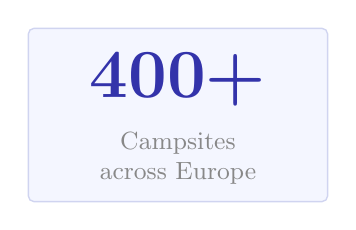
\begin{tikzpicture}
      \node[fill=cardblue,draw=cardborder,line width=0.5pt,
            rounded corners=2pt,minimum width=3.8cm,minimum height=2.2cm] {};
      \node[font=\fontsize{28}{28}\selectfont\bfseries\color{beamerblue}] at (0,0.45) {400+};
      \node[font=\small\color{lightgray},align=center] at (0,-0.55)
        {Campsites\\across Europe};
    \end{tikzpicture}
  \end{column}
  \begin{column}{0.33\textwidth}
    \centering
    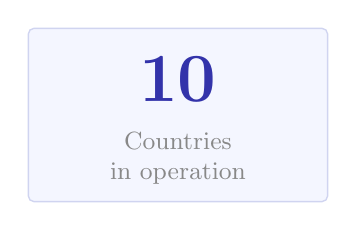
\begin{tikzpicture}
      \node[fill=cardblue,draw=cardborder,line width=0.5pt,
            rounded corners=2pt,minimum width=3.8cm,minimum height=2.2cm] {};
      \node[font=\fontsize{28}{28}\selectfont\bfseries\color{beamerblue}] at (0,0.45) {10};
      \node[font=\small\color{lightgray},align=center] at (0,-0.55)
        {Countries\\in operation};
    \end{tikzpicture}
  \end{column}
  \begin{column}{0.33\textwidth}
    \centering
    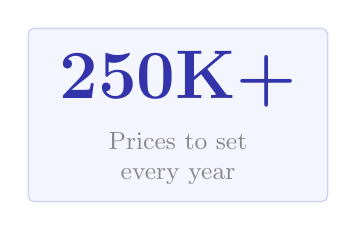
\begin{tikzpicture}
      \node[fill=cardblue,draw=cardborder,line width=0.5pt,
            rounded corners=2pt,minimum width=3.8cm,minimum height=2.2cm] {};
      \node[font=\fontsize{24}{24}\selectfont\bfseries\color{beamerblue}] at (0,0.45) {250K+};
      \node[font=\small\color{lightgray},align=center] at (0,-0.55)
        {Prices to set\\every year};
    \end{tikzpicture}
  \end{column}
\end{columns}

\vspace{1em}
\centering
{\small\itshape\color{lightgray} ROMGID = campsite $\times$ accommodation $\times$ market $\times$ arrival week}

\vspace{0.8em}

\begin{tikzpicture}
  \node[fill=cardblue,draw=beamerblue,line width=1pt,rounded corners=2pt,
        inner sep=8pt,text width=11cm,align=center]
    {\color{beamerblue}\bfseries Can historical booking data recommend better prices
     and increase ECG's revenue?};
\end{tikzpicture}
\end{frame}

% ── SLIDE 4: The Fix ──────────────────────────────────────────────────────────
\begin{frame}{The Fix: Causal Identification}
\vspace{0.5em}
\centering

% Top row: wrong answer left, DAG centre, correct answer right
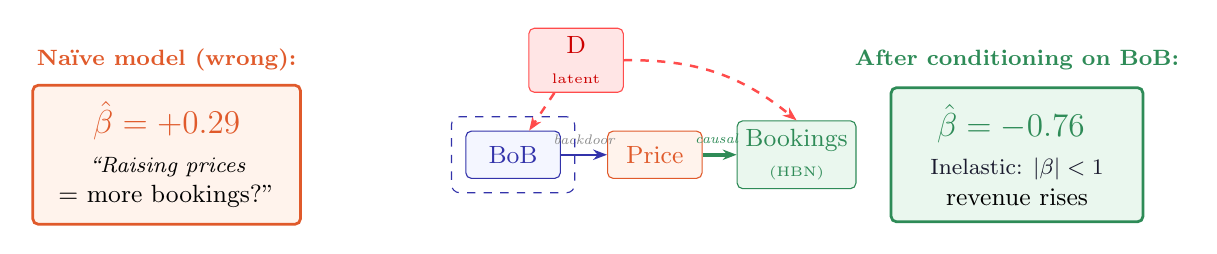
\begin{tikzpicture}[
    every node/.style={font=\small},
    box/.style={draw,rounded corners=2pt,minimum width=1.2cm,
                minimum height=0.6cm,align=center,inner sep=3pt},
    latent/.style={box,draw=red!70,fill=red!10,text=red!80!black},
    bluebox/.style={box,draw=beamerblue,fill=cardblue,text=beamerblue},
    treat/.style={box,draw=accentorange,fill=cardorange,text=accentorange},
    outcome/.style={box,draw=darkgreen,fill=cardgreen,text=darkgreen},
    arr/.style={-{Stealth[length=5pt]},line width=0.9pt},
    redarr/.style={arr,red!70,dashed},
    bluearr/.style={arr,beamerblue},
    greenarr/.style={arr,darkgreen,line width=1.3pt},
  ]

  % Wrong result box (left)
  \node[fill=cardorange,draw=accentorange,line width=1pt,rounded corners=2pt,
        minimum width=3.4cm,minimum height=1.6cm,align=center,inner sep=6pt]
    at (-5.2,0)
    {\color{accentorange}\bfseries\large$\hat\beta = +0.29$\\[3pt]
     \footnotesize\itshape ``Raising prices\\= more bookings?''};
  \node[font=\footnotesize\bfseries\color{accentorange}] at (-5.2, 1.2) {Na\"ive model (wrong):};

  % DAG nodes
  \node[latent] (D) at (0, 1.2) {D\\{\tiny latent}};
  \node[bluebox] (BoB) at (-0.8, 0) {BoB};
  \node[treat]   (p)   at (1.0, 0) {Price};
  \node[outcome] (HBN) at (2.8, 0) {Bookings\\{\tiny(HBN)}};

  % DAG edges
  \draw[redarr] (D) -- (BoB);
  \draw[redarr] (D.east) to[bend left=20] (HBN.north);
  \draw[bluearr] (BoB) -- (p)
    node[midway,above,font=\tiny\itshape,text=lightgray] {backdoor};
  \draw[greenarr] (p) -- (HBN)
    node[midway,above,font=\tiny\itshape,text=darkgreen] {causal $\checkmark$};

  % conditioning box
  \node[draw=beamerblue,dashed,rounded corners=3pt,fit=(BoB),inner sep=5pt] {};

  % Correct result box (right)
  \node[fill=cardgreen,draw=darkgreen,line width=1pt,rounded corners=2pt,
        minimum width=3.2cm,minimum height=1.6cm,align=center,inner sep=6pt]
    at (5.6,0)
    {\color{darkgreen}\bfseries\large$\hat\beta = -0.76\ \checkmark$\\[3pt]
     \footnotesize\color{darktext} Inelastic: $|\beta|<1$\\revenue rises};
  \node[font=\footnotesize\bfseries\color{darkgreen}] at (5.6, 1.2) {After conditioning on BoB:};

\end{tikzpicture}

\vspace{0.5em}
{\small\color{darktext} ECG's pricer reacts to demand: high demand $\to$ prices $\uparrow$, low demand $\to$ prices $\downarrow$.
High prices \& high bookings co-occur in the data $\Rightarrow$ na\"{i}ve regression gets the wrong sign.
Conditioning on BoB closes this backdoor.}

\end{frame}

% ── SLIDE 5: Two Models ───────────────────────────────────────────────────────
\begin{frame}{Two Models, Two Jobs}
\vspace{0.4em}
\begin{columns}[T,onlytextwidth]

%% ── LEFT: Bayesian ──────────────────────────────────────────────────────────
\begin{column}{0.48\textwidth}
\begin{tcolorbox}[
  colback=cardblue, colframe=cardborder,
  arc=3pt, boxrule=0.6pt,
  left=10pt, right=10pt, top=10pt, bottom=10pt
]
  {\bfseries\color{beamerblue} Model v3 $\cdot$ Bayesian}\\[1pt]
  {\footnotesize\itshape\color{lightgray} Goal: estimate elasticity}
  \vspace{10pt}

  \begin{tcolorbox}[
    colback=white, colframe=cardborder,
    arc=2pt, boxrule=0.5pt,
    left=4pt, right=4pt, top=4pt, bottom=4pt
  ]
    \centering
    {\bfseries\color{beamerblue} $\hat\beta = -0.76$}\\[-1pt]
    {\tiny\itshape\color{lightgray} inelastic demand, $|\beta|<1$}
  \end{tcolorbox}
  \vspace{8pt}

  {\footnotesize\color{darktext}
   $\bullet$\ Minimal: only BoB + price\\[4pt]
   $\bullet$\ Cannot make future predictions\\[4pt]
   $\bullet$\ Revenue rises when price rises on average}
\end{tcolorbox}
\end{column}

%% ── RIGHT: LightGBM ─────────────────────────────────────────────────────────
\begin{column}{0.48\textwidth}
\begin{tcolorbox}[
  colback=cardgreen, colframe=greenborder,
  arc=3pt, boxrule=0.6pt,
  left=10pt, right=10pt, top=10pt, bottom=10pt
]
  {\bfseries\color{darkgreen} LightGBM $\cdot$ Gradient Boosting}\\[1pt]
  {\footnotesize\itshape\color{lightgray} Goal: predict \& optimise}
  \vspace{10pt}

  \begin{tcolorbox}[
    colback=white, colframe=greenborder,
    arc=2pt, boxrule=0.5pt,
    left=4pt, right=4pt, top=4pt, bottom=4pt
  ]
    \centering
    {\bfseries\color{darkgreen} $\hat\beta \approx -0.75\ \checkmark$}\\[-1pt]
    {\tiny\itshape\color{lightgray} confirms Bayesian estimate}
  \end{tcolorbox}
  \vspace{8pt}

  {\footnotesize\color{darktext}
   $\bullet$\ Adds lead time \& calendar features\\[4pt]
   $\bullet$\ Out-of-sample error: 27\% per ROMGID\\[4pt]
   $\bullet$\ Flexible demand curve $\to$ interior optima}
\end{tcolorbox}
\end{column}

\end{columns}
\end{frame}

% ── SLIDE 6: Optimiser Results ────────────────────────────────────────────────
\begin{frame}{What the Optimiser Recommends}
\vspace{0.2em}
\begin{columns}[T]

  %% Left: actual histogram from the notebook
  \begin{column}{0.60\textwidth}
  \centering
  {\footnotesize\color{lightgray} Recommended price changes (all snapshots)}\\[2pt]
  \includegraphics[width=\linewidth]{recommendations_distribution.pdf}
  \end{column}

  %% Right: stat cards
  \begin{column}{0.38\textwidth}
  \vspace{0.2em}
  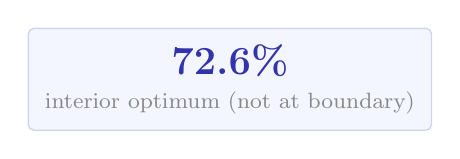
\begin{tikzpicture}
    \node[fill=cardblue,draw=cardborder,line width=0.5pt,rounded corners=2pt,
          minimum width=4.2cm,minimum height=1.1cm,inner sep=6pt,align=center]
      {\color{beamerblue}\bfseries\Large 72.6\%\\
       \footnotesize\color{lightgray} interior optimum (not at boundary)};
  \end{tikzpicture}

  \vspace{0.3em}
  
\begin{tikzpicture}
    \node[fill=cardgreen,draw=greenborder,line width=0.5pt,rounded corners=2pt,
          minimum width=4.2cm,minimum height=1.1cm,inner sep=6pt,align=center]
      {\color{darkgreen}\bfseries\Large \euro63M\\
       \footnotesize\color{lightgray} predicted uplift (+38.8\%)};
  \end{tikzpicture}

  \vspace{0.3em}
  
\begin{tikzpicture}
    \node[fill=cardorange,draw=orangeborder,line width=0.5pt,rounded corners=2pt,
          minimum width=4.2cm,minimum height=1.1cm,inner sep=6pt,align=center]
      {\color{accentorange}\bfseries\Large 51/49\\
       \footnotesize\color{lightgray} green / yellow flag split};
  \end{tikzpicture}

  \vspace{0.4em}
  {\tiny\itshape\color{lightgray} The \euro63M uplift is a model projection and likely optimistic. A randomised experiment is needed.}
  \end{column}

\end{columns}
\end{frame}

% ── SLIDE 7: Next Steps ───────────────────────────────────────────────────────
\begin{frame}{What ECG Should Do Next}
\vspace{1em}

\begin{itemize}\setlength\itemsep{18pt}

  \item[\circlenum{accentorange}{1}]
        {\normalsize\bfseries\color{accentorange} Randomised price experiment}\\[3pt]
        {\small\color{darktext} 100--200 ROMGIDs $\cdot$ prices randomised $\pm$25\% $\cdot$ one 30-week season}\\[2pt]
        {\small\color{lightgray} $\Rightarrow$ unbiased elasticity estimate $\cdot$ tests beyond $\pm$15\% safety range}

  \item[\circlenum{beamerblue}{2}]
        {\normalsize\bfseries\color{beamerblue} Pipeline + dashboard (nightly rerun)}\\[3pt]
        {\small\color{darktext} Recommendations.csv per ROMGID $\cdot$ green/yellow flags $\cdot$ sortable dashboard}\\[2pt]
        {\small\color{lightgray} $\Rightarrow$ builds managerial trust $\cdot$ managers audit anomalies, not all prices}

\end{itemize}

\vspace{0.5em}
\centering{\footnotesize\itshape\color{lightgray} Both tracks run in parallel}
\end{frame}

% ── SLIDE 8: Conclusion ───────────────────────────────────────────────────────
\begin{frame}{Conclusion}
\vspace{0.3em}
\centering

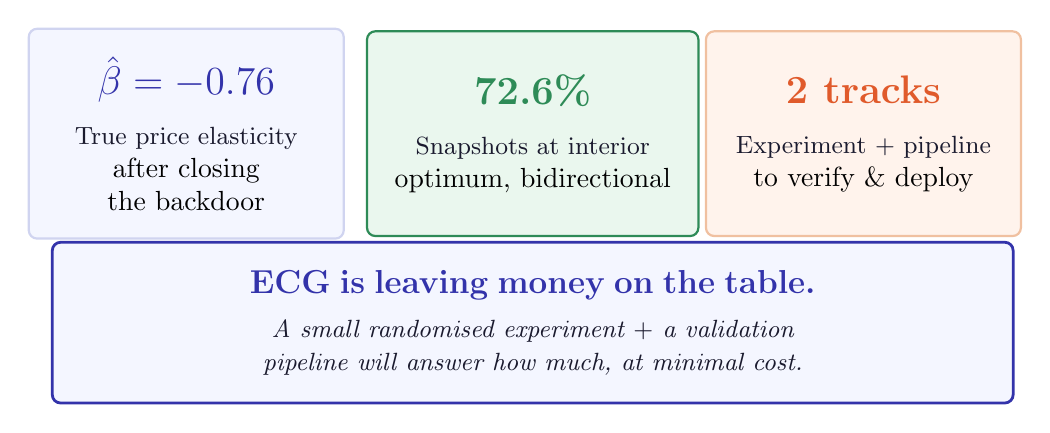
\begin{tikzpicture}
  % Card 1: beta
  \node[fill=cardblue,draw=cardborder,line width=0.8pt,rounded corners=3pt,
        minimum width=4.0cm,minimum height=2.6cm,inner sep=10pt,align=center]
    at (-4.4,0)
    {\color{beamerblue}\bfseries\Large$\hat\beta = -0.76$\\[6pt]
     \small\color{darktext} True price elasticity\\after closing\\the backdoor};

  % Card 2: 72.6%
  \node[fill=cardgreen,draw=greenborder,line width=0.8pt,rounded corners=3pt,
        minimum width=4.0cm,minimum height=2.6cm,inner sep=10pt,align=center]
    at (0,0)
    {\color{darkgreen}\bfseries\Large 72.6\%\\[6pt]
     \small\color{darktext} Snapshots at interior\\optimum, bidirectional};

  % Card 3: 2 tracks
  \node[fill=cardorange,draw=orangeborder,line width=0.8pt,rounded corners=3pt,
        minimum width=4.0cm,minimum height=2.6cm,inner sep=10pt,align=center]
    at (4.2,0)
    {\color{accentorange}\bfseries\Large 2 tracks\\[6pt]
     \small\color{darktext} Experiment + pipeline\\to verify \& deploy};

  % Closing box
  \node[fill=cardblue,draw=beamerblue,line width=1pt,rounded corners=3pt,
        inner sep=10pt,text width=11.5cm,align=center]
    at (0,-2.4)
    {{\color{beamerblue}\bfseries\large ECG is leaving money on the table.}\\[4pt]
     {\small\color{darktext}\itshape A small randomised experiment $+$ a validation pipeline will answer how much, at minimal cost.}};
\end{tikzpicture}

\end{frame}

\end{document}
